\documentclass{report}
\usepackage{fancyhdr} % Required for custom headers
\usepackage{lastpage} % Required to determine the last page for the footer
\usepackage{extramarks} % Required for headers and footers
\usepackage{graphicx} % Required to insert images
%\usepackage{lipsum} % Used for inserting dummy 'Lorem ipsum' text into the template
\usepackage{amsmath}
\usepackage{float}
\usepackage{graphicx} 
%\usepackage{amsfont}
%\usepackage{amssymb}

\usepackage{multicol}
% Margins
\topmargin=-0.5in
\evensidemargin=0in
\oddsidemargin=-0.5in
\textwidth=7.5in
\textheight=9.0in
\headsep=0.25in 


\pagestyle{fancy}

%\rhead{\textbf{Marshall's Recipes}} % Top right header
%\lhead{\textbf{Curry Stir Fry}}
%\chead{ }
%\title{Curry Stir Fry}

\begin{document}
%\vspace{8mm}
%\textbf{PRELIMINARIES:}


\bigskip

\bigskip

\begin{multicols}{2}
\textbf{Ingredients}
\begin{itemize}
\item 1 onion \quad (45 kCal/ 1 gP/ 0 gF/ 11 gC)
\item 1 lbs bacon \quad (2,438 kCal / 170 gP / 187 gF / 6 gC)
\item 3 lbs cubed potatoes \quad (1,041 kCal / 27 gP / 0 gF / 237 gC) 
\item 1 cup heavy cream \quad (469 kCal / 6 gP / 46 gF / 9 gC)
\item 2 cups of milk  \quad (260 kCal / 8 gP / 6 gF / 30 gC)
\item 3 tbsp. butter \quad (306 kCal / 0 gP /36 gF / 0 gC) 
\item $\frac{1}{3}$ cup of flour \quad (152 kCal / 5 gP / 0 gF / 32 gC) 
\item $\frac{2}{3}$ cup sour cream \quad (297 kCal / 5 gP / 45 gF / 7 gC)
\item 1 box chicken broth 
\item 6 cloves minced garlic
\item 1 tsp. chili powder
\item 1 tsp. smoked paprika
\item salt and pepper to taste 


\end{itemize}


\columnbreak
\textbf{Procedure:}
\medskip


\begin{enumerate}
\item \textbf{First, a warning:} This is not a healthy recipe. It is, however, absolutely delicious. 
\item Cut the bacon into small pieces and in a large pot (I use a dutch oven), cook the bacon until crispy. \item Remove the bacon and about half of the remaining bacon grease - I save this for cooking other meals but is not necessary for this recipe. 


\medskip
\item While the bacon cooks, dice your onion, and cube your potatoes into bite-sized pieces. 
\item When you've removed the bacon, cook the onion in the remaining grease and butter until they start turning translucent, then add minced garlic. 

\item When the onion and garlic is fragrant, add in flour and combine. 

\item Add potatoes, broth, milk, cream, paprika, salt, pepper, and bring to an easy boil. If the box of broth isn't enough to cover the potatoes, add water and supplement with bullion. 
\item Cook until potatoes are tender, stirring occasionally to make sure potatoes don't stick to the bottom. 
\item When potatoes are cooked, remove about half the soup and blend. Return the blended mixture to the pot, then add sour cream and bacon. Simmer and stir in the sour cream for another 10 minutes and serve topped with cheese and green onions. 
  
\end{enumerate}
\begin{table}[H]
  \begin{center}
    \caption{Macro totals}
    \label{tab:table1}
    \begin{tabular}{c|c|c|c} % <-- Alignments: 1st column left, 2nd middle and 3rd right, with vertical lines in between
      \textbf{Calories} & \textbf{Protein} & \textbf{Fat} & \textbf{Carbs}\\
      \hline
      5,108 kCal & 222 g & 347 g & 332 g\\
    \end{tabular}
  \end{center}
\end{table}
\end{multicols}




%\begin{center}
%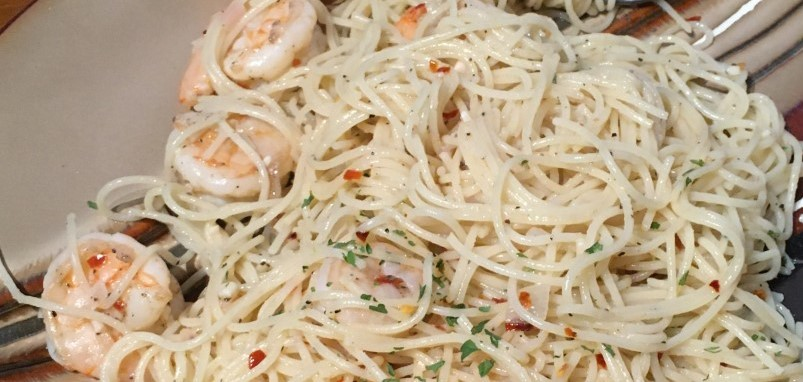
\includegraphics[scale=0.65]{Pasta/Shrimp Scampi/Shrimp Scampi.jpg}
%\end{center}


\end{document}